\documentclass[11pt]{article}

\usepackage[margin=1in]{geometry}
\usepackage{amsmath,amssymb,mathtools}
\usepackage{booktabs}
\usepackage{graphicx}
\usepackage{caption}
\usepackage{microtype}
\usepackage{pdflscape}
\usepackage{hyperref}

\hypersetup{
  colorlinks=true,
  linkcolor=blue,
  urlcolor=blue,
  citecolor=blue,
  pdftitle={Exact High-Dimensional Ehrhart Polynomials and Volumes via Cylindrical Tensor Contraction and Chinese Remainder Reconstruction}
}
\graphicspath{{./}}
\setlength{\emergencystretch}{2em}

\newcommand{\Ocal}{\mathcal{O}}
\newcommand{\Fp}{\mathbb{F}_p}
\newcommand{\Z}{\mathbb{Z}}
\newcommand{\Vol}{\operatorname{Vol}}

\title{Exact High-Dimensional Ehrhart Polynomials and Volumes via Cylindrical Tensor Contraction and Chinese Remainder Reconstruction}
\author{Wendel León Alvarado}
\date{November 11, 2026}

\begin{document}
\maketitle

\begin{abstract}
We present an exact algorithm for Ehrhart counts, Ehrhart $h^*$-polynomials,
and normalized volumes of order polytopes associated with cylindrical
multilayer crown posets.  The algorithm contracts one layer at a time using
axis-wise suffix sums over $\Fp$, then reconstructs integer counts by the
Chinese Remainder Theorem (CRT).  An exact per-dilation bound,
$L_{k,n}(m)\leq (m+1)^{kn}$, determines a sufficient number of 61-bit
primes.  Gradedness supplies the palindromic $h^*$ symmetry, so only the
independent half of the Ehrhart data and one exact symmetry check are needed;
the complete sequence $L_{k,n}(0),\ldots,L_{k,n}(kn)$ is then evaluated from
the reconstructed polynomial.  Experiments cover dimensions 6 through 40.
At dimension 40, Tensor-CRT returns the exact simplex count
$7.8624\times 10^{19}$ in 43.355 seconds with a 52.84 MB
\texttt{tracemalloc} peak, while direct enumeration of the canonical
unimodular triangulation reaches its 15-second cutoff.
\end{abstract}

\noindent\textbf{Keywords:}
Ehrhart polynomial; order polytope; exact counting; tensor contraction;
Chinese Remainder Theorem; high-dimensional computation.

\section{Introduction}

Exact lattice-point enumeration in a high-dimensional polytope is often
approached by decomposing the polytope into cones or simplices.  For order
polytopes, the canonical triangulation is unimodular and is indexed by the
linear extensions of the defining poset.  This gives a conceptually simple
exact baseline, but the number of simplices is the number of linear
extensions and can grow rapidly.  In our experiments, enumerating this
decomposition takes 14.069 seconds already at dimension 16 and exceeds a
15-second cutoff from dimension 20 onward.

We study the cylindrical crown poset $C_{k,n}$, with $k$ layers of $n$
vertices and dimension $d=kn$.  Rather than materializing its triangulation,
we exploit the local cover relations and contract a dense $n$-dimensional
boundary tensor.  Modular arithmetic keeps each tensor entry in a fixed
61-bit field, and CRT recovers exact integers.  This separates working
storage from the number of simplices: the algorithm never stores the
$H_{k,n}(1)$ simplices.

The paper reports a benchmark of nine instances up to $d=40$.  The available
environment did not contain the Normaliz executable, the LattE \texttt{count}
executable, or PyNormaliz; consequently, no direct timing comparison with
those packages is claimed.  The polyhedral baseline reported below is an
exact enumeration of linear extensions, stopped after 15 seconds.  For
timed-out instances, the exact simplex count is independently supplied by
the Tensor-CRT value $H_{k,n}(1)$.

\section{Problem definition and Ehrhart data}

For $k\geq 2$ and $n\geq 3$, let
\[
  C_{k,n}=\{x_{j,i}:1\leq j\leq k,\ i\in\Z/n\Z\}
\]
with cover relations
\[
  x_{j,i}\prec x_{j+1,i},
  \qquad
  x_{j,i}\prec x_{j+1,i+1}
  \quad (1\leq j<k),
\]
where the second index is cyclic.  The order polytope is
\[
  \Ocal(C_{k,n})=
  \{z\in[0,1]^{kn}: z_u\leq z_v\text{ whenever }u\leq v\}.
\]
It is a $d$-dimensional lattice polytope with $d=kn$.  Its Ehrhart count and
$h^*$-polynomial satisfy
\begin{equation}
  L_{k,n}(m)=|m\Ocal(C_{k,n})\cap\Z^d|,
  \qquad
  \sum_{m\geq0}L_{k,n}(m)t^m
  =\frac{H_{k,n}(t)}{(1-t)^{d+1}},
  \qquad
  H_{k,n}(t)=\sum_{j=0}^{r}h_j^*t^j.
  \label{eq:ehrhart}
\end{equation}

The poset is graded: every maximal chain has $k$ elements.  The codegree of
its order polytope is $k+1$, and hence
\[
  r=\deg H_{k,n}=d-k=k(n-1).
\]
The order polytope is Gorenstein, so its $h^*$-polynomial is palindromic in
its actual degree:
\begin{equation}
  h_j^*=h_{r-j}^*=h_{d-k-j}^*
  \quad (0\leq j\leq r).
  \label{eq:palindromic}
\end{equation}
The index is $d-k-j$, not $d-j$: the degree is $d-k$, rather than $d$.
The benchmark reconstructs the independent half by exact triangular
inversion and checks one additional CRT sample against
\eqref{eq:palindromic} for every instance.

\section{Algorithmic architecture}

\subsection{Cylindrical layer transfer}

Fix a dilation $m$ and write $N=m+1$.  Each layer is a vector
$a=(a_0,\ldots,a_{n-1})\in\{0,\ldots,m\}^n$.  Define $F_1(a)=1$ and, for
$q\geq1$,
\begin{equation}
  F_{q+1}(a)=
  \sum_{b\in\{0,\ldots,m\}^n}
  \left(\prod_{i=0}^{n-1}
  \mathbf{1}\{a_i\leq b_i,\ a_i\leq b_{i+1}\}\right)F_q(b),
  \label{eq:transfer}
\end{equation}
with indices modulo $n$.  The two cover inequalities imply that the
coordinate $b_i$ has lower bound
\[
  \ell_i(a)=\max(a_i,a_{i-1}).
\]
Thus the transition can be written
\begin{equation}
  F_{q+1}(a)=
  \sum_{\substack{b_i\geq\ell_i(a)\\0\leq i<n}}F_q(b).
  \label{eq:orthant}
\end{equation}
After $k-1$ transitions,
\[
  L_{k,n}(m)=\sum_{a\in\{0,\ldots,m\}^n}F_k(a).
\]

For a tensor $F$ indexed by $\{0,\ldots,m\}^n$, compute its multidimensional
suffix sum
\[
  S(t_0,\ldots,t_{n-1})
  =\sum_{b_0\geq t_0,\ldots,b_{n-1}\geq t_{n-1}}F(b).
\]
It is obtained by one one-dimensional suffix scan along each axis.  The
transition is then just
$F_{q+1}(a)=S(\ell_0(a),\ldots,\ell_{n-1}(a))$.  A direct pairwise layer
sum would cost $O(N^{2n})$ per transition; axis-wise scans and the indexed
gather cost $O(nN^n)$.  All scans, gathers, and reductions are performed
modulo a prime $p$.

\subsection{CRT bounds and exact reconstruction}

The count is nonnegative and is at most the number of all assignments to
$d$ vertices:
\begin{equation}
  0\leq L_{k,n}(m)\leq(m+1)^d.
  \label{eq:countbound}
\end{equation}
If $p_1,\ldots,p_s$ are distinct 61-bit primes and
$P=\prod_{\nu=1}^s p_\nu>(m+1)^d$, the residues uniquely determine
$L_{k,n}(m)$ in $[0,P)$.  A uniform bound sufficient for every
$0\leq m\leq d$ is
\[
  P>(d+1)^d=(d+1)^{kn}.
\]
The implementation uses the sharper per-dilation bound in
\eqref{eq:countbound}; therefore the reported prime count is the maximum
needed for the independent samples, not the count for a uniform
worst-case bound at $m=d$.

Let $r=d-k$.  The binomial-basis identity from
\eqref{eq:ehrhart} is
\begin{equation}
  L_{k,n}(m)=\sum_{j=0}^{\min(m,r)}
    h_j^*\binom{m+d-j}{d}.
  \label{eq:binomial}
\end{equation}
It gives the triangular recurrence
\begin{equation}
  h_m^*=L_{k,n}(m)-
  \sum_{j=0}^{m-1}h_j^*\binom{m+d-j}{d}.
  \label{eq:triangular}
\end{equation}
We compute CRT counts through
$m=\lfloor r/2\rfloor+1$, use \eqref{eq:triangular} for the first half, and
use \eqref{eq:palindromic} for the remaining coefficients.  The extra
sample tests the middle symmetry coefficient exactly.  Finally,
\eqref{eq:binomial} evaluates all integer counts $L_{k,n}(0),\ldots,
L_{k,n}(d)$ exactly.  Thus not every one of these $d+1$ values requires an
independent tensor contraction.

\subsection{Volumes and the canonical triangulation}

The value at one is
\[
  H_{k,n}(1)=\sum_{j=0}^{r}h_j^*.
\]
For an order polytope this is also the number of linear extensions, and
therefore the number of unimodular simplices in its canonical
triangulation.  Since every simplex has Euclidean volume $1/d!$,
\begin{equation}
  \Vol(\Ocal(C_{k,n}))=\frac{H_{k,n}(1)}{d!}.
  \label{eq:volume}
\end{equation}
Equation~\eqref{eq:volume} is reported as a reduced exact rational number.

\section{Complexity and memory}

Let $N_{\max}$ be one plus the largest CRT dilation used.  A modular
transition costs $O(nN_{\max}^n)$ word operations: $n$ axis scans and an
$O(n)$ coordinate-index calculation per tensor entry.  It is repeated over
$k-1$ layers, at most $O(kn)$ independent dilations, and
$O(\log M)$ primes, where $M=(d+1)^d$ is the uniform count bound.  Since
$N_{\max}\leq d+1=kn+1$, the contraction work is bounded by
\[
  O\!\left(k^2n^2(kn+1)^n\log M\right),
\]
which in particular is within the requested conservative bound
\begin{equation}
  O\!\left(k^2n^3(kn+1)^n\log M\right).
  \label{eq:complexity}
\end{equation}
The triangular $h^*$ inversion adds $O(d^2)$ exact integer operations.
These are arithmetic-operation bounds; bit complexity additionally
accounts for the $O(\log M)$-bit exact counts and CRT intermediates.

The implementation stores the current and next $N_{\max}^n$ residue
tensors, with chunk-sized index vectors for the gather.  Its working
storage is $O(N_{\max}^n)$ machine words (plus the bit length of exact
integer outputs), independent of the number $H_{k,n}(1)$ of simplices.
In particular, it does not allocate a simplex list.  A dense 64-bit
coordinate array for the explicit triangulation would require
$H_{k,n}(1)(d+1)d\cdot8$ bytes; at $d=40$ this is
$1.0315\times10^{24}$ bytes, compared with a measured Tensor-CRT
\texttt{tracemalloc} peak of 52.84 MB.

\section{Experimental benchmark through dimension 40}

All measurements were produced by
\texttt{benchmark\_ehrhart\_d40.py}.  Tensor-CRT wall time includes the
independent CRT contractions and exact polynomial reconstruction.  Peak
memory is measured with Python's \texttt{tracemalloc}.  The polyhedral
column is a recursive exact enumeration of canonical linear extensions,
terminated after 15 seconds.  A timeout is a censored observation $>15$ s,
not a completed baseline time.  The exact simplex count in every row is
$H_{k,n}(1)$ from the exact numerator.  Normaliz, LattE, and PyNormaliz
were not installed in the benchmark environment.

\begin{landscape}
\begin{center}
\captionsetup{hypcap=false}
\captionof{table}{Exact Tensor-CRT and canonical triangulation benchmark.
Volumes are reduced rational numbers.}
\label{tab:benchmark}
\small
\setlength{\tabcolsep}{4pt}
\renewcommand{\arraystretch}{1.15}
\resizebox{\linewidth}{!}{%
\begin{tabular}{@{}rrrrrrrl@{}}
\toprule
$(k,n)$ & $d$ & CRT primes & Tensor-CRT (s) & Peak (MB) &
Polyhedral baseline & $H_{k,n}(1)$ & Euclidean volume exact \\
\midrule
$(2,3)$ & 6  & 1 & 0.013 & 0.01 & 0.346 s & 48 & \texttt{1/15} \\
$(3,3)$ & 9  & 1 & 0.021 & 0.01 & 0.565 s & 384 & \texttt{1/945} \\
$(3,4)$ & 12 & 1 & 0.025 & 0.08 & 0.589 s & 50,688 & \texttt{1/9450} \\
$(4,4)$ & 16 & 1 & 0.062 & 0.25 & 14.069 s & 2,363,392 & \texttt{577/5108103000} \\
$(4,5)$ & 20 & 2 & 0.412 & 6.11 & \texttt{TIMEOUT $>15$ s} & 4,957,143,040 & \texttt{3782/1856156927625} \\
$(5,5)$ & 25 & 2 & 1.579 & 15.19 & \texttt{TIMEOUT $>15$ s} & 1,759,112,069,120 & \texttt{521/4593988395871875} \\
$(6,5)$ & 30 & 2 & 4.900 & 32.21 & \texttt{TIMEOUT $>15$ s} & 624,279,871,815,680 & \texttt{97921/41606059170426672796875} \\
$(7,5)$ & 35 & 3 & 17.339 & 40.00 & \texttt{TIMEOUT $>15$ s} & 221,547,727,526,297,600 & \texttt{6388/297940989719425403898421875} \\
$(8,5)$ & 40 & 3 & 43.355 & 52.84 & \texttt{TIMEOUT $>15$ s} & 78,624,058,898,424,791,040 & \texttt{615124/6383403244813084051148273014453125} \\
\bottomrule
\end{tabular}%
}
\end{center}
\end{landscape}

\begin{figure}[htbp]
  \centering
  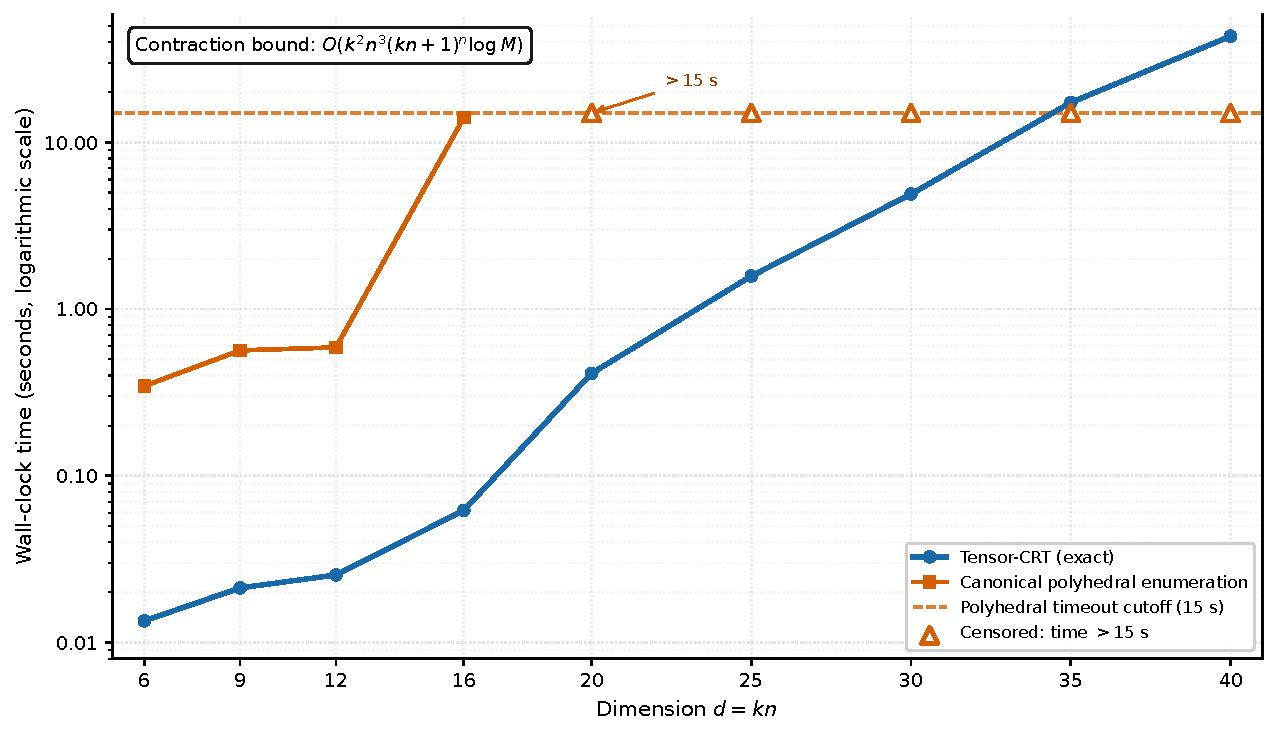
\includegraphics[width=0.94\linewidth]{fig_tiempos_d40.pdf}
  \caption{Wall-clock comparison on a logarithmic scale. Triangles denote
  right-censored polyhedral enumeration at the 15-second cutoff. The
  asymptotic Tensor-CRT operation bound is shown in the annotation.}
  \label{fig:times}
\end{figure}

\begin{figure}[htbp]
  \centering
  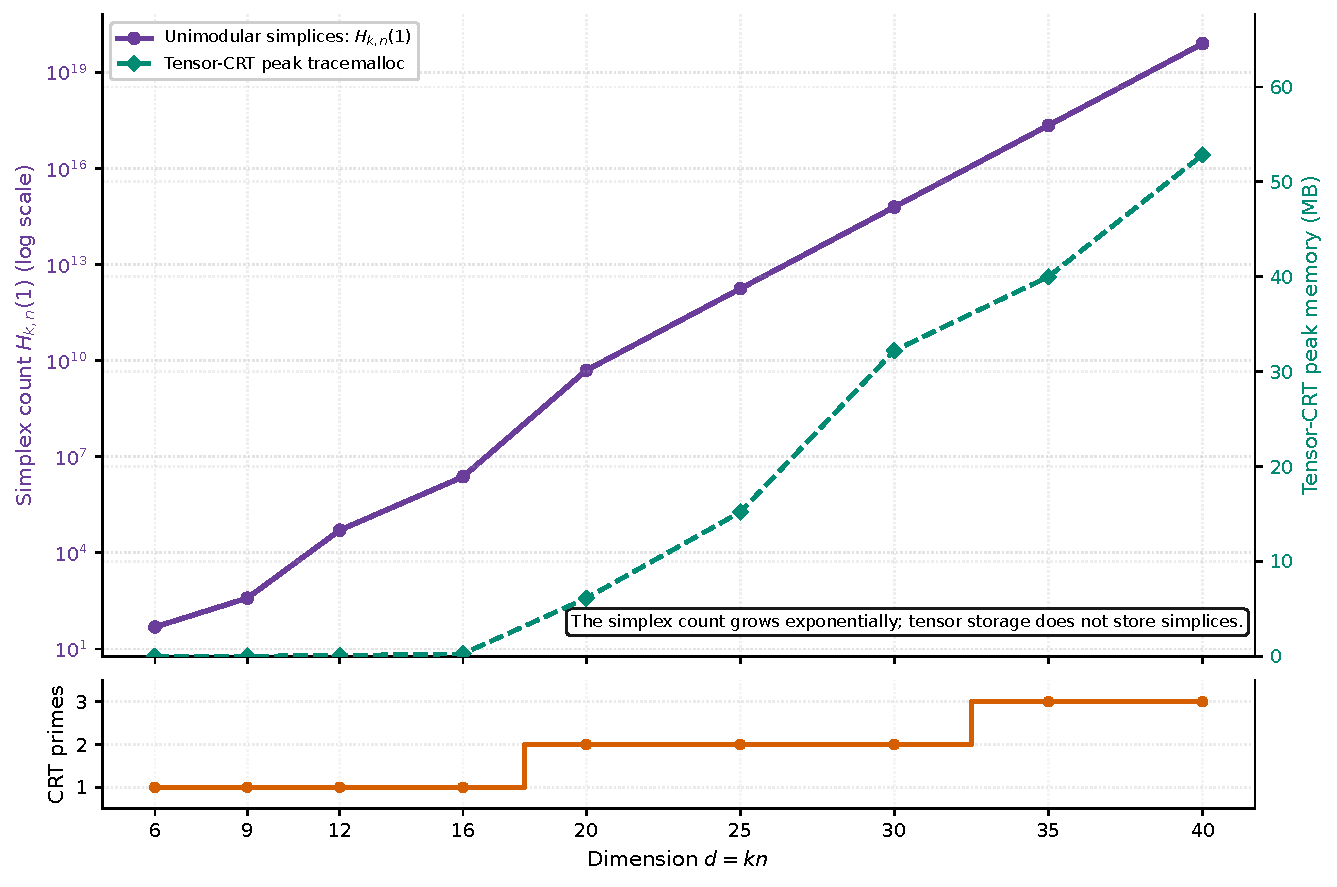
\includegraphics[width=0.94\linewidth]{fig_memoria_simplices_d40.pdf}
  \caption{Exact number of canonical unimodular simplices, Tensor-CRT peak
  memory, and the number of 61-bit CRT primes used for the independent
  dilations.}
  \label{fig:memory}
\end{figure}

Figure~\ref{fig:times} shows that the exact tensor contraction completes all
nine cases, while direct triangulation enumeration reaches the cutoff from
$d=20$.  Figure~\ref{fig:memory} shows the separation between the rapidly
growing simplex count and the tensor workspace: from $d=6$ to $d=40$,
$H(1)$ grows from 48 to $7.8624\times10^{19}$, while measured peak memory
grows from 0.01 MB to 52.84 MB.  The maximum number of CRT primes needed for
the independent reconstruction samples is three.  The reported $h^*$
vectors are palindromic in degree $d-k$, and the extra exact CRT sample
agrees with that symmetry in each instance.

\section{Conclusion and reproducibility}

Cylindrical layer contraction replaces explicit triangulation by exact
multidimensional suffix scans, and CRT converts bounded modular
computations back to integer Ehrhart data.  The benchmark reaches dimension
40 while keeping the contraction workspace far below the memory required
to store the corresponding triangulation explicitly.

The implementation, source benchmark data, figure generator, vector and
300-dpi raster figures, and this manuscript are colocated in
\texttt{BENCHMARK\_D40/}.  Reproduce the figures with
\texttt{python generar\_graficas.py}; compile this manuscript twice with
\texttt{pdflatex -interaction=nonstopmode -halt-on-error
paper\_tensor\_crt.tex}.  The next algorithmic extension is to replace the
two-neighbor cylindrical cover pattern by local constraints on more
general periodic graphs while retaining a bounded-width tensor boundary.

\begin{thebibliography}{9}
\bibitem{BeckRobins}
M. Beck and S. Robins,
\emph{Computing the Continuous Discretely: Integer-Point Enumeration in
Polyhedra}, 2nd ed., Springer, 2015.

\bibitem{Stanley}
R. P. Stanley,
Two poset polytopes,
\emph{Discrete \& Computational Geometry} 1 (1986), 9--23.
\end{thebibliography}

\end{document}
